% vim:ft=tex:
%
\documentclass[12pt]{article}

\title{
	alternate_domain_diag
}
\author{
	bolster --- \texttt{bolster@milo}
}
\usepackage{pgfplots}

\begin{document}

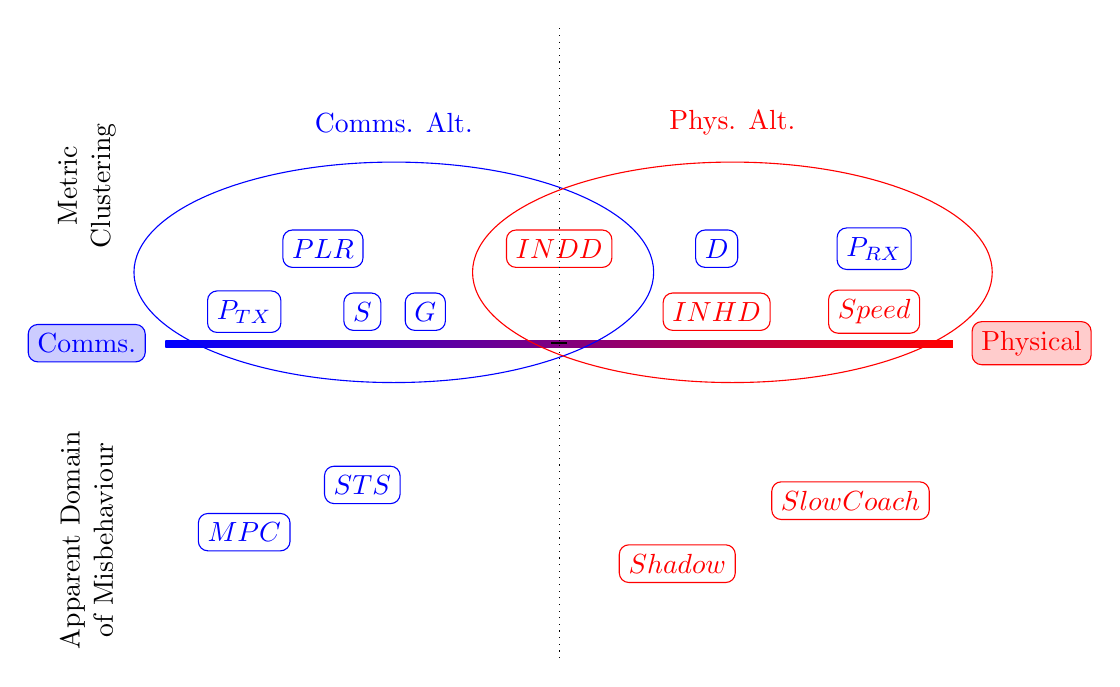
\begin{tikzpicture}[-latex,
  comms/.style={text=blue, draw=blue, rounded corners=.8ex},
  phys/.style={text=red, draw=red, rounded corners=.8ex}]
  % Start off with the line
  %\draw [<-|][comms, draw=blue, very thick] (0,1) -- (5,1); 
  %\draw [|->][phys, draw=red, very thick] (5,1) -- (10,1); 
  \path[left color=blue,right color=red]
  (0,0.95) rectangle +(10,2.5pt);

  % Baseline labels
  \node[comms, fill=blue, fill opacity=0.2, text opacity=1] at (-1,1) {Comms.};
  \node[phys, fill=red, fill opacity=0.2, text opacity=1] at (11,1) {Physical};
  
  % Metric Labels
  \node[comms] at (7,2.2) {$D$};
  \node[comms] at (9,2.2) {$P_{RX}$};
  \node[comms] at (1,1.4) {$P_{TX}$};
  \node[comms] at (2.5,1.4) {$S$};
  \node[comms] at (3.3,1.4) {$G$};
  \node[comms] at (2,2.2) {$PLR$};
  \node[phys] at (5,2.2) {$INDD$};
  \node[phys] at (7,1.4) {$INHD$};
  \node[phys] at (9,1.4) {$Speed$};

  \node[rotate=90, align=center] at (-1, 3) {Metric\\Clustering};
  \node[rotate=90, align=center] at (-1, -1.5) {Apparent Domain\\of Misbehaviour};
  \node[comms] at (1,-1.4) {$MPC$};
  \node[comms] at (2.5,-0.8) {$STS$};
  \node[phys] at (6.5,-1.8) {$Shadow$};
  \node[phys] at (8.7,-1) {$SlowCoach$};

  % Draw approx subsets
  \draw[comms] (2.9,1.9) ellipse (3.3 and 1.4);
  \draw[phys] (7.2,1.9) ellipse (3.3 and 1.4);

  \node[text=red] at (7.2,3.8) {Phys. Alt.};
  \node[text=blue] at (2.9,3.8) {Comms. Alt.};

  % Misc
  \draw[-|][dotted] (5,5) -- (5,1);
  \draw[-|][dotted] (5,-3) -- (5,1);


\end{tikzpicture}

\end{document}
